\documentclass{beamer}

% This file is a solution template for:

% - Talk at a conference/colloquium.
% - Talk length is about 20min.
% - Style is ornate.



% Copyright 2004 by Till Tantau <tantau@users.sourceforge.net>.
%
% In principle, this file can be redistributed and/or modified under
% the terms of the GNU Public License, version 2.
%
% However, this file is supposed to be a template to be modified
% for your own needs. For this reason, if you use this file as a
% template and not specifically distribute it as part of a another
% package/program, I grant the extra permission to freely copy and
% modify this file as you see fit and even to delete this copyright
% notice. 


\mode<presentation>
{
    \usetheme{Warsaw}
  % or ...

    \setbeamercovered{transparent}
  % or whatever (possibly just delete it)
}


\usepackage[english]{babel}
\usepackage{verbatim}
\usepackage{graphicx}
% or whatever

\usepackage[latin1]{inputenc}
% or whatever

\usepackage{times}
\usepackage[T1]{fontenc}
% Or whatever. Note that the encoding and the font should match. If T1
% does not look nice, try deleting the line with the fontenc.


\title
{Indirect Control Flow Analysis}

\subtitle
{Discovering possible ICF targets}

\author
{LIU Xuebao}
% - Give the names in the same order as the appear in the paper.
% - Use the \inst{?} command only if the authors have different
%   affiliation.

\institute
{Institue of Computing Technology}
% - Use the \inst command only if there are several affiliations.
% - Keep it simple, no one is interested in your street address.

%\date[CFP 2003] % (optional, should be abbreviation of conference name)
%{Conference on Fabulous Presentations, 2003}

% - Either use conference name or its abbreviation.
% - Not really informative to the audience, more for people (including
%   yourself) who are reading the slides online

%\subject{Theoretical Computer Science}
% This is only inserted into the PDF information catalog. Can be left
% out. 



% If you have a file called "university-logo-filename.xxx", where xxx
% is a graphic format that can be processed by latex or pdflatex,
% resp., then you can add a logo as follows:

% \pgfdeclareimage[height=0.5cm]{university-logo}{university-logo-filename}
% \logo{\pgfuseimage{university-logo}}



% Delete this, if you do not want the table of contents to pop up at
% the beginning of each subsection:
\AtBeginSubsection[]
{
    \begin{frame}<beamer>{Outline}
        \tableofcontents[currentsection,currentsubsection]
    \end{frame}
}


% If you wish to uncover everything in a step-wise fashion, uncomment
% the following command: 

%\beamerdefaultoverlayspecification{<+->}


\begin{document}

\begin{frame}
    \titlepage
\end{frame}

\begin{frame}{Outline}
    \tableofcontents
  % You might wish to add the option [pausesections]
\end{frame}

\section{What are ICF?}

\subsection{Definition}

\begin{frame}{Definition}
    \begin{block}{Definition}
        \emph{\textbf{I}ndirect \textbf{C}ontrol \textbf{F}low} indicates that
        the targets of control-flow transfers are determined at \alert{runtime}.
    \end{block}

    \begin{block}{Key point}
        Instruction pointer is determined at runtime.
    \end{block}
\end{frame}

\subsection{Classification}

\begin{frame}{Classification}
    \begin{itemize}
        \item
            Indirect control-flow transfer Instuructions(ICFTI): CALL and JMP
        \item
            Indirect control-flow transfer Functions(ICFTF): setjmp() and sigsetjmp()
        \item
            Signal and Interrupt (???)
    \end{itemize}
\end{frame}

\section{Methodology}
\subsection{Where to find the possible ICF targets?}

\begin{frame}{Characteristics of ICFTI targets}
    \begin{itemize}
        \item
            A \alert{register} or \alert{memory} pointer specifies the ICF
            targets.
            \pause
        \item
            Before used as targets, the registers or memories shall be
            initialized.
            \pause
        \item
            Most of the initializers(targets) could be found in \alert{Code Segment} or
            \alert{Data Segment} directly.
            \pause
        \item
            A few targets could be obtained by simple arithmetic compution on
            initializers.
    \end{itemize}
\end{frame}

\begin{frame}{Characteristics of ICFTF targets}
    \begin{itemize}
        \item
            Usually, the targets are addresses of the instructions, which are
            the successors of insturctions \emph{CALL} to setjmp/sigsetjmp.
            \pause
        \item
            How to find the insturctions \emph{CALL} to setjmp/sigsetjmp?
    \end{itemize}
\end{frame}

\subsection{How to discover the possible ICF targets?}

\begin{frame}{Discover the possible ICF targets}
    \begin{itemize}
        \item MOV \textbf{imm}, reg/mem
            --- The immidiate is a candidate target.
            \pause
        \item LEA \textbf{imm(RIP)}, reg
            --- The (immididate+RIP) is a candidate target.
            \pause
        \item LEA+
            --- If X is a candidate target in LEA format, X+MEM(X) is a candidate target.
            \pause
        \item data
            --- Any 8-byte numerics, which meet the constrants, is a candidate target.
        \item rodata
            --- Any 8-byte numerics, which meet the constrants, is a candidate target.
            \pause
        \item got, ctros and dtors
            --- Entries in \emph{.got}, \emph{.ctros} and \emph{.dtors} are candidate targets.
    \end{itemize}
    
\end{frame}

\begin{frame}[fragile]{Category I -- MOV}
    \begin{block}{Format}
        MOV \textbf{imm}, reg \\
        MOV \textbf{imm}, mem
    \end{block}

    \begin{exampleblock}{Example}
        \begin{verbatim}
0000000000402a90 <_start>:
    ...
  402a9f:	mov    $0x5b4ac0,%r8
  402aa6:	mov    $0x5b4ad0,%rcx
  402aad:	mov    $0x402bf0,%rdi
  402ab4:	callq  402620 <__libc_start_main@plt>
    ...
        \end{verbatim}
    \end{exampleblock}
\end{frame}

\begin{frame}[fragile]{Category II -- LEA}
    \begin{block}{Format}
        LEA \textbf{imm(RIP)}, reg
    \end{block}

    \begin{exampleblock}{Example}
        \begin{verbatim}
    ...
  404c3d:	lea    0x2e(%rip),%r11  # 404c72 
  404c44:	sub    %rax,%r11
  404c47:	lea    0xbf(%rsp),%rax
  404c4f:	jmpq   *%r11
    ...
  404c6e:	movaps %xmm0,-0x7f(%rax)
  404c72:	mov    %rsi,%r14
    ...
        \end{verbatim}
    \end{exampleblock}
\end{frame}

\begin{frame}[fragile]{Category III -- LEA+}
    \begin{block}{Format}
        LEA \textbf{imm(RIP)}, reg
    \end{block}

    \begin{exampleblock}{Example}
        \begin{verbatim}
    ...
  5af47e:	lea    0xeb(%rip),%r11  # 5af570
    ...
  5af48c:	mov    (%r11,%r9,8),%r10
  5af490:	lea    (%r10,%r11,1),%r11
  5af494:	jmpq   *%r11
  5af497:	mov    (%rdx),%r11b
    ...
  5af4bd:	mov    (%rdx),%r10w
    ...
        \end{verbatim}
    \end{exampleblock}
\end{frame}

\begin{frame}[fragile]{Category IV -- data}
    \begin{exampleblock}{Example}
        \textbf{842b70} e0004500 00000000 \alert{70094100 00000000}\\
        \textbf{842b80} f0004500 00000000 f0014500 00000000
        \begin{verbatim}
    ...
0000000000410970 <Perl_pp_pushmark>:
  410970:	push   %r12
  410972:	push   %rbx
  410973:	push   %rsi
    ...
        \end{verbatim}
    \end{exampleblock}
\end{frame}

\begin{frame}[fragile]{Category V -- rodata}
    \begin{exampleblock}{Example}
        \textbf{5bda60} 46864000 00000000 31864000 00000000 \\
        \textbf{5bda70} 1c864000 00000000 07864000 00000000 \\
        \textbf{5bda80} \alert{f7854000} 00000000 00000000 00000000
        \begin{verbatim}
    ...
  4085f7:	mov    0x0(%r13),%rcx
  4085fb:	mov    %rcx,0x44499e(%rip)
  408602:	jmpq   40b30c
  408607:	mov    0x0(%r13),%rdi
  40860b:	callq  40cd80 <Perl_scope>
  408610:	mov    %rax,0x444989(%rip)
  408617:	jmpq   40b30c
  40861c:	mov    0x0(%r13),%rdi
    ...
        \end{verbatim}
    \end{exampleblock}
\end{frame}

\subsection{How to reduce false negative?}

\begin{frame}{Constraints}
    \begin{itemize}
        \item
            Candidate targets (exclude those from got, ctors and dtors) must
            not point to the destinations outside the current module.
            \pause
        \item
            Candidate targets must not point to destinations inside any one
            instruction.
            \pause
        \item
            \ldots
    \end{itemize}
\end{frame}

\section{Evaluation}
\begin{frame}{Evaluation}
    \begin{itemize}
        \item Benchmarks
            \begin{itemize}
                \item 4 programs of SPEC2006
            \end{itemize}
        \item Compiler
            \begin{itemize}
                \item icc
            \end{itemize}
        \item Platform
            \begin{itemize}
                \item X86\_64 GNU/Linux
            \end{itemize}
    \end{itemize}
\end{frame}

\begin{frame}{Results}
    \begin{figure}[htbp]
        \centering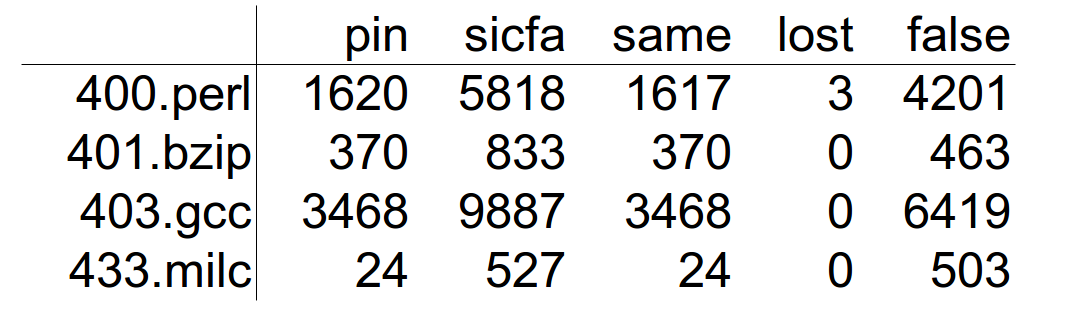
\includegraphics[width=0.8\textwidth]{results.png}
    \end{figure}
\end{frame}

\section{Conclusion}
\begin{frame}{Conclusion}
    \begin{itemize}
        \item
            A static analysis for indirect control-flow targets is useful.
            \pause
        \item Challenges
            \begin{itemize}
                \item Subset and superset \pause
                \item Obfuscation of Executable Code
            \end{itemize}

    \end{itemize}
\end{frame}

\begin{frame}
    \Huge{\centerline{The End}}
\end{frame}
\end{document}


